%%%%%%%%%%%%%%%%%%%%%%%%%%%%%%%%%%%%%%%%%%%%%%%%%%%%%%%%%%%%%%%%%%%%%%%%%%%%%%%%
% experiment.tex: Chapter describing the experiment
%%%%%%%%%%%%%%%%%%%%%%%%%%%%%%%%%%%%%%%%%%%%%%%%%%%%%%%%%%%%%%%%%%%%%%%%%%%%%%%%
\chapter{The CMS Detector}
\label{sec:experiment_chapter}
%%%%%%%%%%%%%%%%%%%%%%%%%%%%%%%%%%%%%%%%%%%%%%%%%%%%%%%%%%%%%%%%%%%%%%%%%%%%%%%%
The energies and trajectories of charged leptons and jets produced in proton-proton (pp) collisions are measured so 
that the masses \mWR and \mnul can be determined.  The maximum \mWR and \mnul that can be measured are constrained by 
the pp collision energy and collision intensity integrated over time.  The mass resolutions are driven by the 
resolutions with which the lepton and jet energies and trajectories are measured.  In this chapter, the CERN Large 
Hadron Collider (LHC) and the pp collisions it delivers are described as a prelude to the main topic of the chapter - 
the Compact Muon Solenoid (CMS) sub-detectors that are used to identify leptons and jets, and measure their energies 
and trajectories.  The structure and the performance of the sub-detectors used to detect leptons and jets are described 
here, and a more detailed explanation is given elsewhere \cite{cmsDetectorPaper}.


\section{The LHC and CMS Overview}
\label{sec:lhcCmsOverview}
The LHC was constructed in a 27 km circular tunnel \cite{lhcTDR} to deliver pp collisions at 13 $\TeV$.  In the 
collider two proton beams that contained $\sim$2300 proton bunches, with 25 ns separating adjacent 
bunches are collided at the center of the CMS detector.  Collisions occurred at 4 interaction points (IPs), and 
the beam optics were such that the highest intensity collisions occurred at 2 IPs.  The general purpose ATLAS 
(A Toroidal Lhc Apparatus) \cite{atlasTdrPhysPerformance} and CMS \cite{cmsTdrPhysPerformance} 
experiments were built around these IPs, and the CMS IP coincides with the geometric center of CMS.  The interaction 
intensity $\Ell$, given by Equation \ref{eq:instLumi}, is inversely proportional to the product of the two beam areas 
$4\pi \epsilon_{n}\beta^{*}$, and proportional to a geometric factor F based on the beam crossing angle, and the rate 
of protons crossing the IP $fnN^{2}\gamma$.  The interaction frequency f is fixed at 40 MHz by the time separating 
adjacent bunches, the Lorentz boost $\gamma$ is fixed by the beam energy, and the factor F is fixed by the LHC design.  
The other parameters - the number of bunches n, the number of protons per bunch N, and the beam areas - are manipulated 
to maximize the interaction intensity $\Ell$.  In 2015 the intensity at the CMS IP approached $6 \times 10^{33} \frac{Hz}{cm^{2}}$ 
($6 \times 10^{-3} \frac{Hz}{pb}$), and the intensity integrated over the year was 2.6 fb$^{-1}$ \cite{lumi}.

\begin{equation}
	\Ell = \frac{fnN^{2}\gamma}{4\pi \epsilon_{n}\beta^{*}}F
\label{eq:instLumi}
\end{equation}

Particles produced at the CMS IP were detected using the sub-detectors shown in Figure \ref{fig:layersOfCMS}.  Located closest 
to the IP was the silicon tracker, which was used to detect and track charged particles.  Surrounding the tracker were the electromagnetic 
(ECAL) and hadronic (HCAL) calorimeters, which were used to identify and measure the kinematics of photons and electrons (e$^{\pm}$), 
and neutral and charged hadrons.  The tracker and both calorimeters were inside a solenoid magnet that generated a 3.8 $\unit{T}$ 
magnetic field.  Muon detectors were located in the iron magnet return yoke where the magnetic field strength varied between 
1 and 3 $\unit{T}$, and were used to detect and track muons ($\mu^{\pm}$) over several meters.  Each sub-detector covered 360$^{\circ}$ 
in the plane perpendicular to the beam axis, and was divided into a barrel and two endcap sections to detect particles over a large 
angular region: between 5.65$^{\circ}$ and 90$^{\circ}$ away from the beam axis.

Particles detected in each sub-detector were characterized by energies perpendicular to the beam axis and trajectories relative 
to the IP.  The tracker and muon detectors measured the scalar transverse momentum ($\pt$) of particles, and the calorimeters 
measured their scalar transverse energy ($\Et$).  Detected particles were assumed to be massless, so $\pt$ and $\Et$ were equivalent.  
Each particle's trajectory was represented by a vector pointing from the IP to the spatial position of an energy 
measurement, and the vector coordinates were expressed in terms of two quantities: the angle $\phi$, $0 \leq \phi < 2\pi$, in 
the plane perpendicular to the beam direction, and the pseudorapidity $\eta$:

\begin{equation}
	\eta \equiv \frac{1}{2}\ln{\frac{E+p_{z}}{E-p_{z}}}
\end{equation}
where E is the magnitude of the particle's energy, and $p_{z}$ is the particle's momentum along the beam direction.  The 
transverse energies $\Et$ and $\pt$ are related to the magnitudes $E$ and $|p|$ by $\Et \equiv E/\cosh{\eta}$ and 
$\pt \equiv |p|/\cosh{\eta}$.  The quantities $\eta$ and $\phi$ were also used to quantify the distance between two 
trajectories as $\Delta R \equiv \sqrt{\eta^{2} + \phi^{2}}$.  Finally, each particle detected in the tracker was also 
distinguished by a point of origin - an interaction vertex.  Each vertex's position was measured from the IP, and was 
defined by a transverse distance perpendicular to the beam axis, and a longitudinal distance along the beam axis.

\begin{figure}[h]
	\centering
	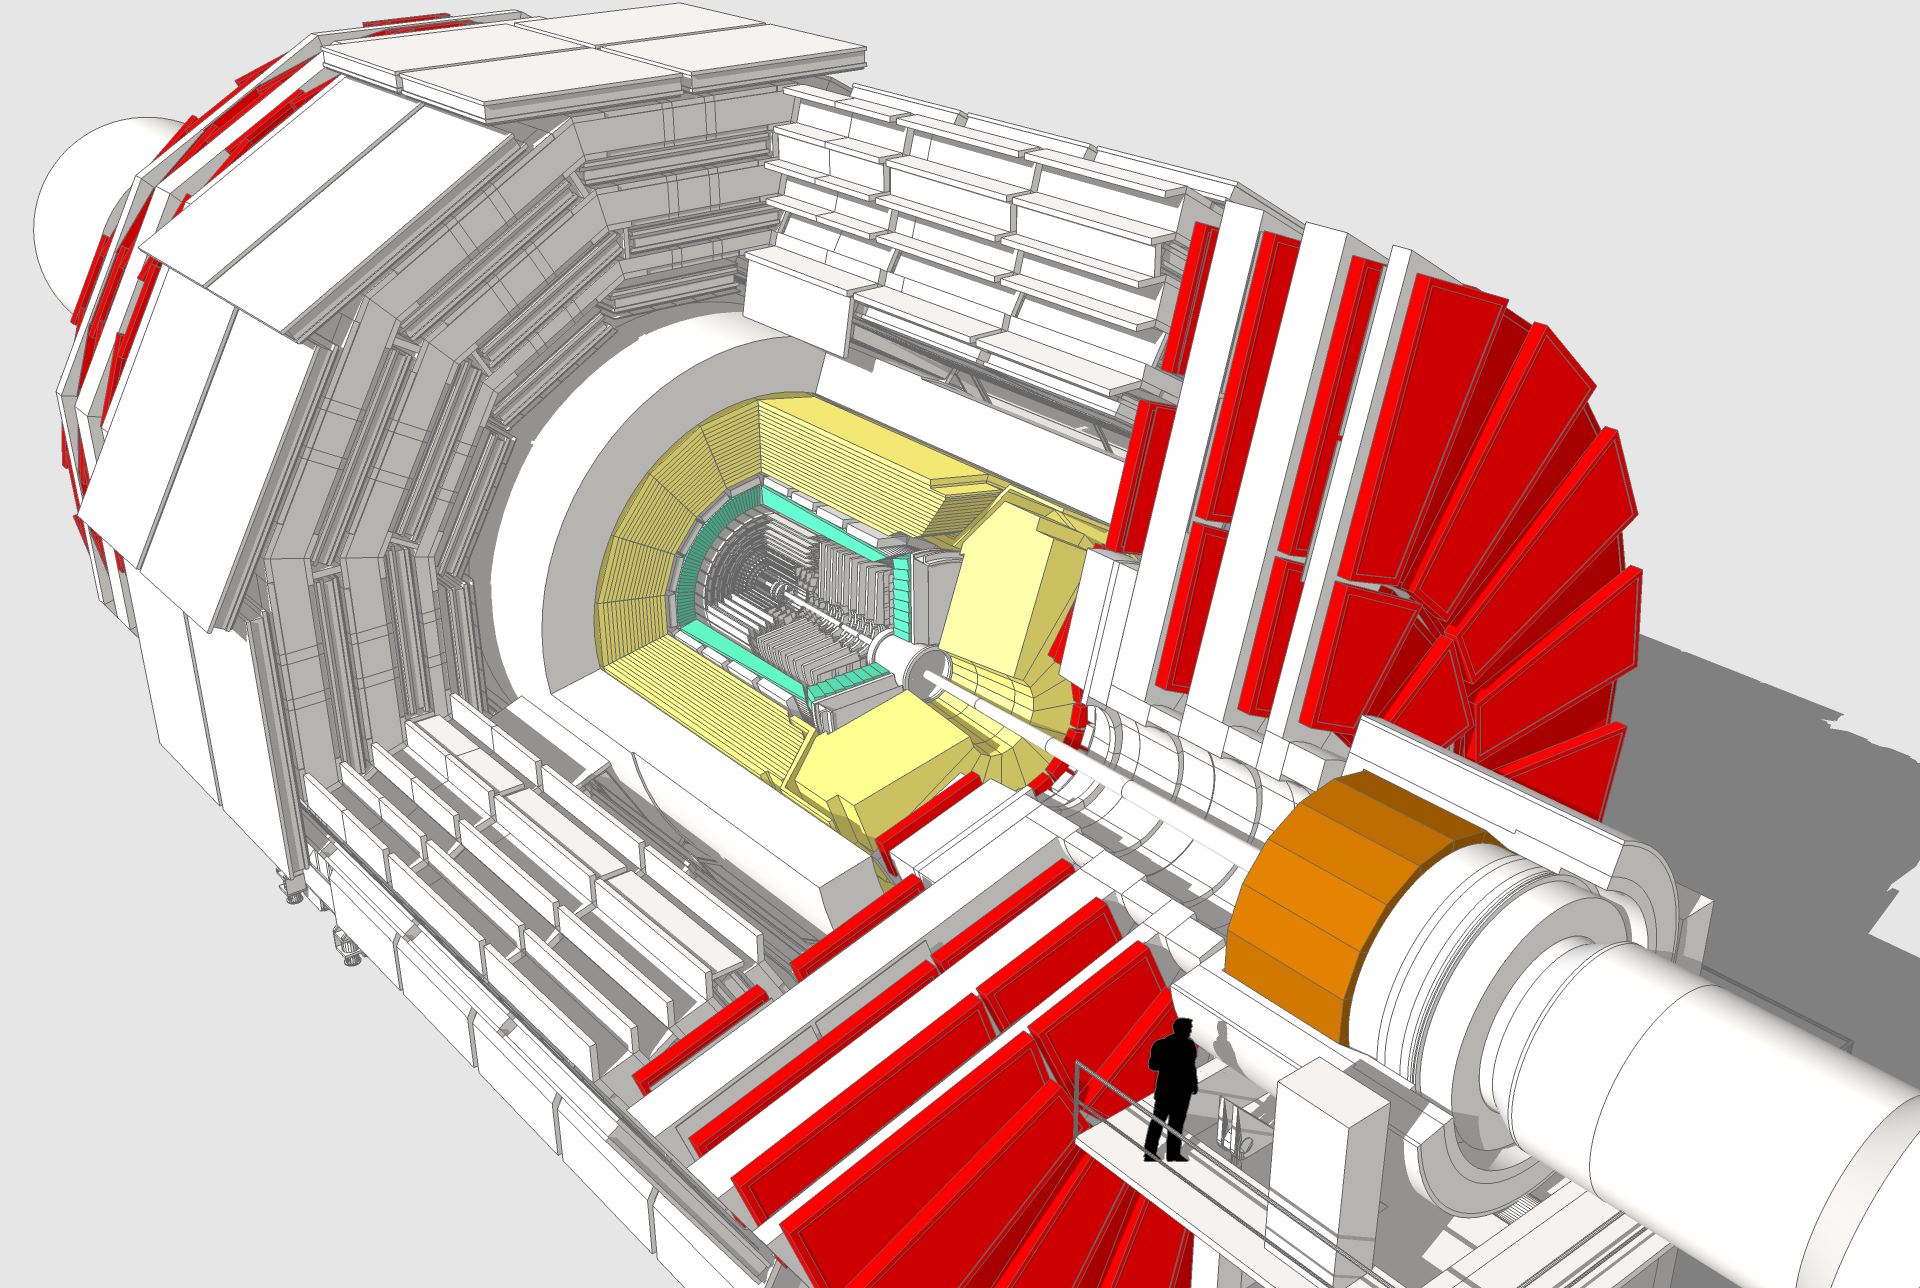
\includegraphics[width=1\textwidth]{figures/cmsDetectorBasic.png}
	\caption{Cut-away view of the entire CMS detector.  Closest to the proton-proton interaction point is the 
		silicon tracker, followed by the electromagnetic calorimeter, then the hadronic calorimeter, and the 
	magnet.  The muon detectors are located in the magnet iron return yoke.}
	\label{fig:layersOfCMS}
\end{figure}

\section{The Silicon Tracker}
\label{sec:siTrackerDescription}
The silicon tracker consisted of silicon pixel and strip detectors whose purpose was to detect and track charged particles 
as they traverse the magnetic field, thereby measuring their radii of curvature.  Then the points where particle tracks 
originated were used to identify interaction vertices.  Closest to the beam axis was the pixel detector, which used 
silicon pixels to measure particles' points of origin and their trajectories up to 15 cm from the $z$ axis.  Surrounding 
the pixel detector was the strip detector, which used silicon strips to measure the radii of curvature of particles up to 
110 cm from the $z$ axis.

The pixel tracker was built from $\approx$1 m$^{2}$ of arrays of pixels, each covering 100 $\times$ 150 $\mu$m$^{2}$.  In 
the barrel region ($0 < |\eta| < 1.2$), individual silicon detectors were assembled in three concentric cylindrical shells 
centered on the $z$ axis.  In the endcap region ($1.2 < |\eta| < 2.5$), two layers of pixel detectors were installed in a 
turbine pattern (Figure \ref{fig:pixelTracker}) \cite{pixelCommissioning}.  These provided up to 3 measurements for every 
track, and primarily were used to reconstruct interaction vertices.

\begin{figure}[ht]
	\centering
	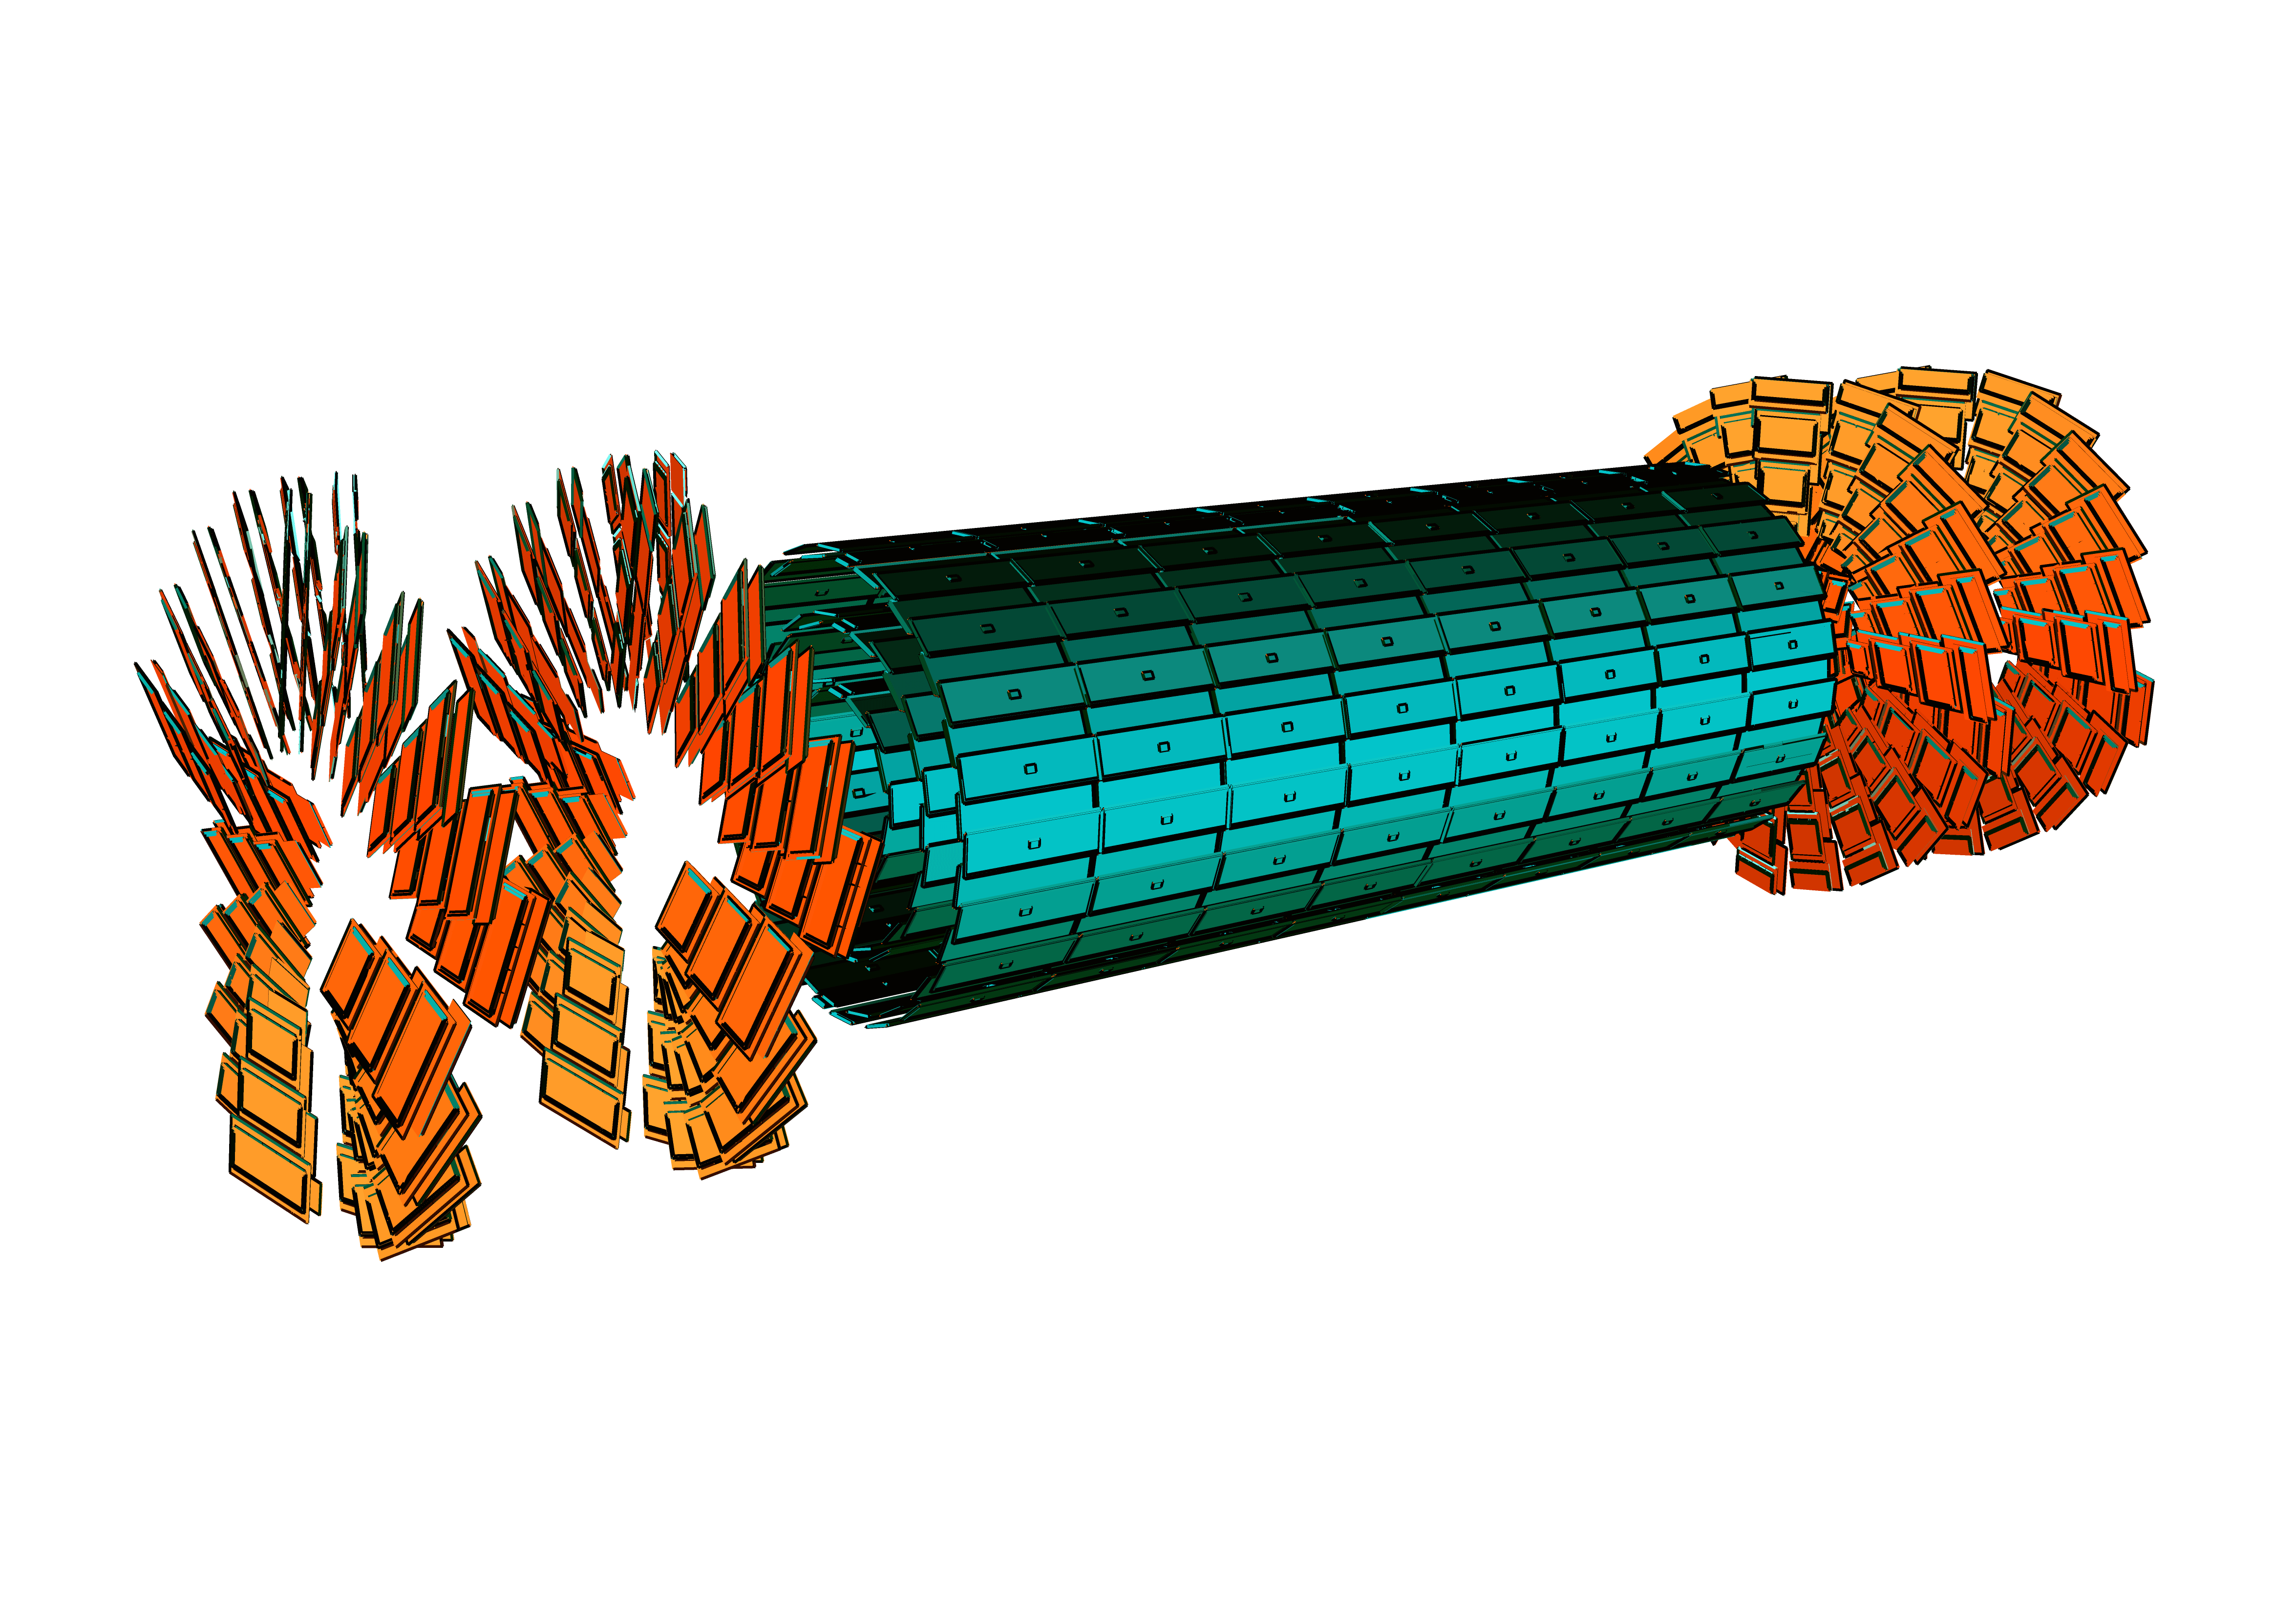
\includegraphics[width=0.8\textwidth]{figures/pixelDetectorSchematic.png}
	\caption{The barrel and endcap sections of the pixel detector.}
	\label{fig:pixelTracker}
\end{figure}

Located outside the pixel tracker, the strip tracker was constructed with 198 m$^{2}$ of silicon divided into arrays of strips, 
and organized into four structures based on $|\eta|$ and distance from the IP.  As the distance from the beam axis increased, the 
strip width increased from 80 to 180 $\mu$m, and the strip length increased from 12 to 16 cm.  
In the barrel region, silicon strips were used to build 10 concentric cylindrical shells.  In the endcap region, silicon 
strips were arranged in 12 disks, as shown in Figure \ref{fig:stripTracker} \cite{cmsTDR}, with some overlap in $|\eta|$ with 
the barrel region silicon strips.  The strip tracker provided between 5 and 14 measurements for every track over a $\sim$1 meter 
distance.

\begin{figure}[ht]
	\centering
	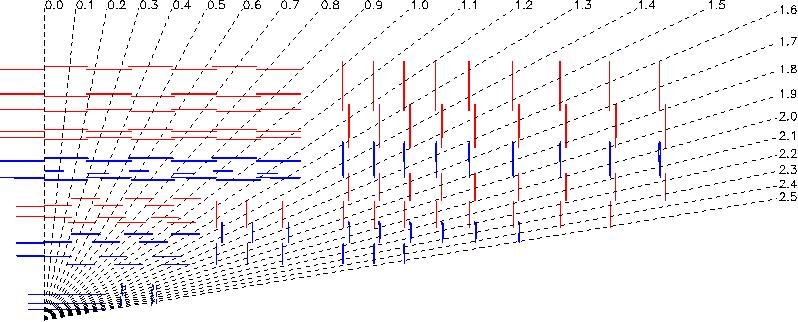
\includegraphics[width=0.8\textwidth]{figures/siliconStripAndPixelDetectorTwoDimView.png}
	\caption{The barrel and endcap sections of the strip detector for $\eta \geq 0.$ and one quadrant of $\phi$.  
	The pixel detector is shown to scale in the bottom left corner.}
	\label{fig:stripTracker}
\end{figure}

Charged particles traversing the tracker generated signals in silicon detector modules that each had arrays of pixels or strips 
connected to Read-Out Chips (ROCs).  In the pixel tracker, each ROC was connected to an array of 52 $\times$ 80 pixels.  The pixel 
tracker barrel was built from silicon detector modules that each had 16 ROCs.  In the pixel tracker endcap, each turbine blade was 
built from 7 silicon detector modules (4 on one face, 3 on the other), and each module had between 2 and 10 ROCs.  In total, 
$\sim$16000 ROCs were connected to 66 million pixels.  The strip tracker used a different type of ROC, and each ROC was connected 
to 128 strips located on the same $\eta$ ring.  Each ROC and its associated strips was one strip detector module, and the strip 
tracker was built from $\sim$15400 detector modules.

The tracker measured the positions and energies of charged particles at up to 17 points, and as far as 1.1 meters from the beam 
axis.  The track reconstruction algorithms, described later, identified sets of track points as individual particle tracks.  Along 
the trajectory of each track, the equation of motion of a charged particle in an inhomogenous magnetic field subject to ionization 
energy losses in silicon was solved numerically.  The numerical solution was used to extract the particle's radius of curvature, and 
thereby its $\pt$.

The tracker performance depended on the number and momenta of the charged particles in a collision event.  In events where two leptons 
and jets were reconstructed from tracks that pointed to one vertex, the vertex's position was measured with a resolution better than 
12$\mu$m in any direction \cite{trackerPerformanceInCollisions}.  
The tracker measured charged particle momenta by measuring the radius of curvature of charged particle tracks; thus 
the $\pt$ resolution degraded with increasing $\pt$.  For muons with $20 < \pt < 100$ $\GeV$, the 
tracker measured the $\pt$ of barrel region muons with a resolution of 1.3\% to 2.0\%, and measured the $\pt$ of endcap muons 
with a resolution of 6\% or better \cite{muonRecoFirstCollisions}; higher $\pt$ muons were measured with a worse $\pt$ resolution.  
Charged hadrons that did not undergo a nuclear interaction in the tracker were measured with a $\pt$ resolution similar that of a 
muon.  Accounting for the $\eta$-dependent tracker material budget of 0.18 to 0.56 nuclear interaction lengths, the tracker measured 
the $\pt$ of all charged hadrons with $10 < \pt < 100$ $\GeV$ with a resolution of 3.3\% or better in the barrel, and 20\% or better 
in the endcap \cite{trackerPerformanceInCollisions}.  Electrons were detectable as tracks if they had $\pt > 0.4$ $\GeV$ and 
$|\eta| < 2.5$, but their $\pt$ resolution was significantly worse than that of charged hadrons or muons due to multiple scattering 
and bremsstrahlung.  The tracker measured the $\pt$ of electrons with $10 < \pt < 100$ $\GeV$ with a resolution of between 6\% and 
27\% of $\pt$ in the barrel, and between 20\% and 50\% of $\pt$ in the endcap.

To measure the positions of the interaction vertices and charged particle momenta with these resolutions, the tracker alignment was 
measured before the start of data taking with cosmic ray muons.  The alignment is the position of the silicon detector modules relative 
to the calorimeters and muon detectors.  Knowing and calibrating the alignment is crucial because the momenta of charged particles 
and the positions of interaction vertices are extracted from track position measurements.  During collisions, $Z \rightarrow \mu\mu$ 
events and cosmic ray muons were used to monitor and recalibrate the tracker alignment.

In the reconstruction, charged leptons and hadrons were distinguished from photons and neutral hadrons using tracks found in the 
tracker.  Tracks that extrapolated to energy deposits found in the electromagnetic calorimeter (ECAL) or hadronic calorimeter (HCAL) 
were identified as electrons or charged hadrons, respectively.  Tracks found in the silicon tracker that extrapolated to tracks found 
in the muon detectors were identified as muons.


\section{The Electromagnetic Calorimeter}
\label{sec:ecalDescription}
Surrounding the silicon tracker was the electromagnetic calorimeter (ECAL), which detected photons, and distinguished electrons and 
positrons from other charged particles.  The ECAL is a homogeneous absorption calorimeter built from scintillating lead-tungstate 
(PbWO$_{4}$) crystals.  In response to incident photons and electrons ($e^{\pm}$), the ECAL crystals emitted visible light in $\sim$20 
ns in amounts proportional to the incident particle energies that was detected with avalanche photodiodes (APDs) and vacuum phototriodes 
(VPTs).

The ECAL contained 75848 crystals \cite{ecalPerformanceInCollisions} divided into barrel and endcap regions.  In the barrel region 
($0 < |\eta| < 1.479$), 61200 crystals with $\sim$26 radiation lengths\footnote{On average the energy of a relativistic $e^{\pm}$ 
decreases by $e^{-1}$ after travelling through one radiation length of material.} of PbWO$_{4}$ were arranged in a cylindrical shell.  
The scintillation light emitted in the barrel crystals was detected with APDs.  The front face of each crystal measured 2.2 $\times$ 
2.2 cm$^{2}$, and was 19 cm away from the outer most silicon tracker layer.  In the endcap region ($1.479 < |\eta| < 3.0$), 14648 crystals 
(half in each endcap) with $\sim$25 radiation lengths of PbWO$_{4}$ were installed in a disk.  The scintillation light emitted in the 
endcap crystals was detected with VPTs.  The front face of the endcap crystals measured 2.86 $\times$ 2.86 cm$^{2}$, and was located behind 3 radiation 
lengths of lead and silicon that constituted a preshower detector.  The preshower detector is a sampling calorimeter built from two 
disks of lead absorber and two planes of silicon strips that cover $1.653 < |\eta| < 2.6$.  The first disk is 2 radiation lengths thick, 
and the second is 1 radiation length thick.  The back side of each disk is covered by arrays of silicon sensors that each cover 63 
$\times$ 63 mm$^{2}$ and contain 32 individual strips.  Each silicon sensor was connected to its own Read-Out Chip (ROC), and groups of 
7, 8, or 10 ROCs were organized into individual micromodules.  The preshower detector improved the spatial and energy resolution with 
which electromagnetic showers were studied in the endcap.  A partial view of the ECAL barrel, endcap and preshower detectors is shown 
in Figure \ref{fig:ecalEBEEandES} \cite{ecalTDR}.

\begin{figure}[ht]
	\centering
	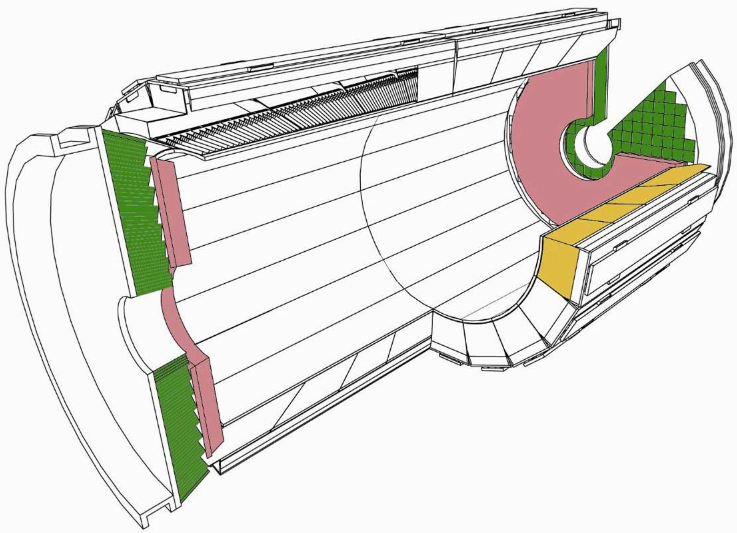
\includegraphics[width=0.8\textwidth]{figures/ecalBarrelEndcapAndPreshower.png}
	\caption{The ECAL barrel, endcap and preshower detectors.}
	\label{fig:ecalEBEEandES}
\end{figure}

The ECAL measured the energies of photons and electrons with $0 < |\eta| < 3.0$ by measuring the amount of scintillation light produced 
in clusters of crystals.  The density of PbWO$_{4}$, 5.4 $\frac{gm}{cm^{3}}$, was sufficiently high that the signal of an electron or 
photon was usually fully contained in a 3 $\times$ 3 crystal cluster centered on the most energetic crystal.  To estimate the energy lost 
through bremsstrahlung in the tracker, the signals of electrons and photons were measured in 3 $\times$ 5 crystal clusters or larger.  Based 
on real collision data, the ECAL measured the energies of electrons from $Z \rightarrow ee$ decays ($\Et \approx 45 \GeV$) with a resolution 
better than 2\% for $|\eta| < 0.8$, and between 2\% and 5\% elsewhere.  At a slightly lower $\Et$ scale in real collision data, the ECAL measured 
the energies of photons from $Z \rightarrow \mu\mu\gamma$ decays with a resolution of 2.5\% in the barrel, and 4.7\% in the endcaps \cite{ecalPerformanceInCollisions}.

To measure photon and electron energies with similar precision across the entire detector, the ECAL crystals were 
monitored and calibrated during data taking using several techniques.  Every 40 minutes each ECAL crystal was illuminated 
with light from blue and green lasers to monitor the crystal transparency.  Every week laser data 
was used to calculate new crystal correction factors, which corrected the changes in crystal transparency 
since the previous week.  Photons from $\eta \rightarrow \gamma\gamma$, and electrons from 
$W \rightarrow e\nu$ and $Z \rightarrow e^{+}e^{-}$ were used to validate the weekly transparency corrections.

To compliment the transparency corrections, additional corrections were applied to ECAL crystals 
to calibrate their responses based on the arrival times and energies of reconstructed particles.  Relative energy 
and arrival time corrections for each crystal were calculated using methods described elsewhere \cite{eGammaMonitCalib2011}, and 
were applied to normalize the the responses of all crystals, in terms of energy and time, to the same value.  Then 
absolute energy scale corrections were derived using electrons from $Z \rightarrow e^{+}e^{-}$ events, and applied 
to calibrate each crystal's energy response to the true $Z$ boson mass.  New arrival time corrections were applied 
every month, and new energy corrections were applied once in September 2015.

In the reconstruction, energies measured by individual ECAL crystals were grouped into dynamically 
sized superclusters (SCs) with at least 15 crystals.  The SC size was allowed to vary in $\eta$ and $\phi$ to capture 
bremsstrahlung photons produced when $e^{\pm}$s traversed the silicon tracker.  In the subset of SCs that were isolated 
from HCAL energy deposits, each $e^{\pm}$ was identified as a SC that geometrically matched a reconstructed track 
trajectory, and each photon was identified as a SC not matched to any track.


\section{The Hadronic Calorimeter}
\label{sec:hcalDescription}
Surrounding the ECAL was the hadronic calorimeter (HCAL), which detected charged and neutral hadrons.  The 
HCAL is a sampling calorimeter constructed with 17 layers of 3.7 mm thick scintillating plastic tiles separated by 
17 layers of 5 cm thick metal absorber plates.  In the barrel 
region ($0 < |\eta| < 1.4$), absorber plates and scintillating tiles were organized into 2304 towers, each 
covering a 5 $\times$ 5 grid of ECAL barrel crystals.  In the endcap region ($1.3 < |\eta| < 3.0$), absorber 
plates and scintillating tiles were assembled into 2304 towers (1152 per endcap), each covering 
a 5 $\times$ 5 grid of ECAL endcap crystals.

Hadrons that impinged on the HCAL showered in brass absorber layers, and in $\sim$10 ns produced scintillation 
light in the plastic tiles.  Optical fibers transmitted the scintillation light to hybrid photodiodes, 
which measured the scintillation light to determine the energies of incident hadrons.  The HCAL was used in 
combination with the tracker, ECAL, and muon detectors to measure the energy of jets.  After calibrating the 
HCAL and the other sub-detectors, the energy of jets with $\pt > 40\GeV$ and $|\eta| < 1.3$ was measured with 
a resolution of 16\% or better \cite{jetResolutionInCollisions}.

To measure hadron energies with similar precision across the whole detector, the amount of light measured in scintillating tile towers 
was monitored and calibrated before and during 2015 collisions.  Before collisions, a cesium-137 source 
was lowered into the HCAL, and the amount of scintillation light produced by each 
tower was used to calibrate each tower's response.  Once collisions began, a laser system 
monitored the efficiency of light transmission from the scintillator tiles to the photodetectors.  
From laser transparency data, relative calibrations were derived that normalized the energy response of all towers 
to the same level.  The absolute energy calibration was determined in events where a jet recoiled off a photon, or 
a leptonically decaying Z boson.  There, the absolute hadronic energy 
scale was calibrated relative to the electromagnetic or muonic energy scale derived from $Z \rightarrow \ell\ell$ 
and $Z \rightarrow \mu\mu\gamma$ events.  Finally, the precision of the absolute hadronic energy scale calibration 
was improved using dijet resonances like $W/Z \rightarrow jj$.

In the reconstruction, the energy measured by each HCAL tower was treated as the basic unit of HCAL energy.  
Each reconstructed hadron contained at least one HCAL energy deposit, and potentially one or more ECAL energy 
deposits.  Reconstructed tracks that extrapolated to the $(\eta,\phi)$ positions of HCAL energies were identified 
as charged hadrons, while HCAL energies that did not match any track were identified as neutral hadrons.


\section{The Muon Detectors}
\label{sec:muonDetectorsDescription}
Interspersed among layers of the magnet iron return yoke were gas ionization chambers that were used to detect and measure the 
trajectories of muons.  The muon detectors had a geometrical acceptance of $0 < |\eta| < 2.4$.  Since the muon detectors were 
located 4.0 meters or further from the IP, the muon detectors also measured each muon's arrival time to identify the collision 
event that produced it.

The muon barrel and endcap sections, shown in Figure \ref{fig:muonBarrelAndEndcapDetectors}, used three types of gas ionization 
detectors to identify muons and to measure their kinematics.  In the barrel region ($0 < |\eta| < 1.2$), drift tubes (DTs) and 
resistive plate chambers (RPCs) were used, while in the endcap region ($1.2 < |\eta| < 2.4$), RPCs and cathode strip chambers 
(CSCs) were used.

\begin{figure}[ht]
	\centering
	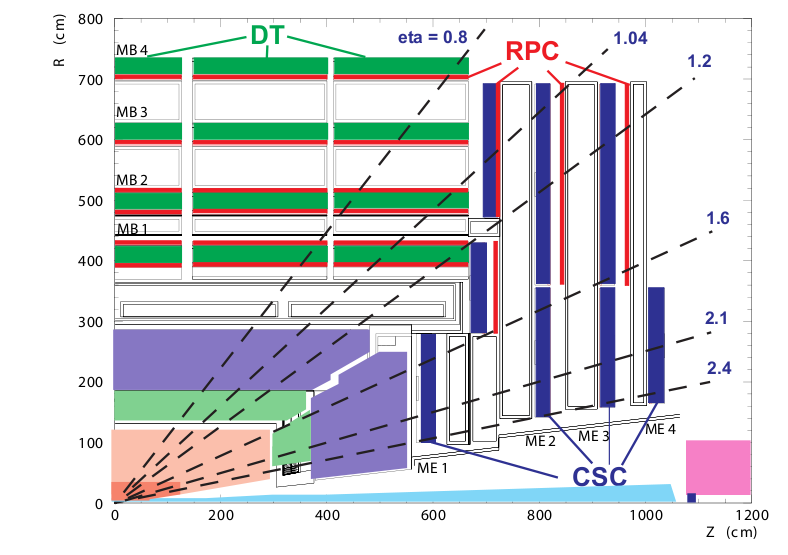
\includegraphics[width=0.8\textwidth]{figures/muonDetectorLayout.png}
	\caption{The barrel and endcap sections of the muon detectors for $\eta \geq 0.$ and one quadrant of $\phi$.  Shown 
		between the muon detectors and the interaction point are the magnet solenoid and return yoke, the HCAL, the ECAL, 
		and the silicon tracker.}
	\label{fig:muonBarrelAndEndcapDetectors}
\end{figure}

The DTs were organized into 5 wheels, each with 4 radial units called stations, and 12 $\phi$ segments per 
station that each covered 30 degrees in $\phi$.  Each DT chamber measured muon trajectories using a set of 4 DT 
planes measuring r-z coordinates\footnote{There were no r-z planes of drift tubes in the outermost station.} that 
were between two sets of DTs measuring r-$\phi$ coordinates.  Each r-$\phi$ set had 4 DT planes, and the two sets 
were separated by 24 cm to increase the lever arm length that causes muons to curve in the magnetic field.  Based on 
collision data from 2015, each DT station measured muon trajectories with a resolution better than 300$\mu$m in any 
direction, and measured muon arrival times with a resolution of 2 ns \cite{cmsMuonRecoRunTwo}.  

In the endcap, CSCs were installed in four disks facing the interaction point.  These disks were segmented into several radial layers 
(rings of different radii, stations), as shown in Figure \ref{fig:muonBarrelAndEndcapDetectors}, each containing 18 or 36 chambers, 
and each chamber had 6 planes of CSC detectors.  Based on muon measurements made in 2015, the CSC chambers measured muon trajectories 
with a resolution better than 150 $\mu$m in any direction, and measured muon arrival times with a resolution of 3.2 ns \cite{cmsMuonRecoRunTwo}.

In the barrel and endcap for $|\eta| < 1.9$, the RPCs measured muon arrival times with a resolution better than 2 ns.  RPC measurements 
were used to identify the collision event that produced each muon \cite{cmsMuonRecoRunTwo}.

By combining information from the tracker and the muon system, the $\pt$ resolution of muons could be improved.  Due to the 3.8 
$\unit{T}$ magnetic field, the tracker measured muon momenta in the $\pt <$ 200 $\GeV$ phase space with a resolution better than the 
muon detectors by a factor of 3 or more.  As the muon $\pt$ increased above 200 $\GeV$, the muon momentum resolution reduced.  However, 
since particle trajectories in the muon detectors were measured over 3 meters or more, the $\pt$ of muons with a $\pt > 200$ $\GeV$ was 
measured with a better resolution than the tracker.  Based on cosmic ray measurements made in 2015, the combined tracker and muon system 
measured the $\pt$ of barrel region muons that had $200 < \pt < 400 \GeV$ with a resolution ($\frac{\Delta p}{\pt}$) of 3.5\% or better 
\cite{cmsMuonRecoRunTwo}.

To measure the trajectories of tracks and muon momenta with these resolutions, the muon detector alignment was measured before the 
start of data taking with cosmic ray muons.  Knowing and calibrating the alignment is crucial because the momenta of muons and their 
trajectories are extracted from track position measurements.  During collisions, cosmic ray muons, and $W \rightarrow \mu\nu$ and 
$Z \rightarrow \mu\mu$ events were used to monitor and recalibrate the alignment of the muon detectors.

In the reconstruction, the tracks measured in individual $\phi$ segments of each muon station were treated as the basic building block 
of a muon.  Each reconstructed muon contained one track from a muon station or one track from the silicon tracker, or both.


\section{The Trigger System}
\label{sec:triggerDescription}
In 2015 the rate of pp collision events delivered by the LHC was many orders of magnitude greater than the 
rate that CMS could store all the data.  The LHC collided two proton bunches at a rate of 40 MHz, and in nearly every 
collision $\gtrsim$1 $\GeV$ of energy was detected in CMS.  Due to the large cross section of QCD multijet processes 
and leptonically decaying heavy quark processes (Figure \ref{fig:smProductionXsxns}), there were $\sim10^{6}$ collision 
events per second with energetic charged leptons or hadronic jets.  A two level event-selection trigger system was used 
to select events during collisions (online) that were stored for physics analyses.

\begin{figure}[h]
	\centering
	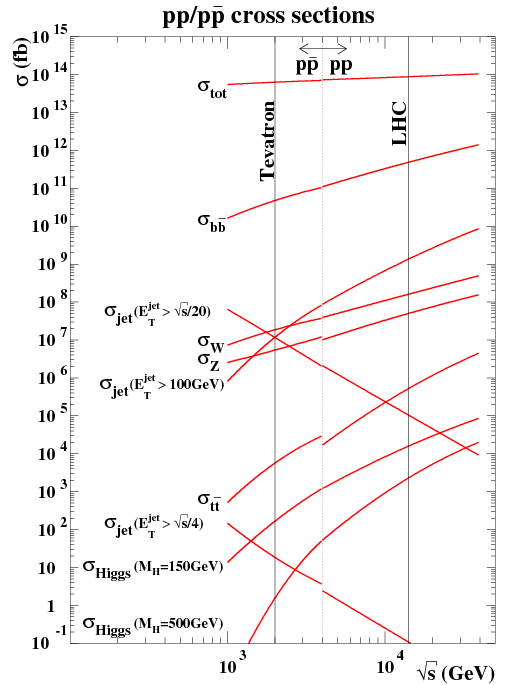
\includegraphics[width=0.6\textwidth]{figures/lhc_and_tevatron_cross_sections_2006.png}
	\caption{Production cross sections at the LHC and Tevatron as a function of center of mass energy.  Each cross section divided by $10^{5}$ yields 
	the approximate production rate in events per second in 2015 at the LHC.}
	\label{fig:smProductionXsxns}
\end{figure}

The Level-1 (L1) trigger system searched for collision events with photons, charged leptons, hadronic 
jets or missing energy.  After every collision event, data from the ECAL, the HCAL and the muon detectors was used to 
identify energy clusters and build tracks that represented photons, hadrons, muons and other particles.  In $\sim$1 $\mu$s these 
clusters and tracks, distinguished by $(\eta, \phi)$ trajectories and $\Et$ (or $\pt$) values, were built and sent to the L1 
logic system located $\sim$20 m from CMS.  Implemented in programmable hardware, the L1 logic system ran $\sim$200 algorithms 
in less than 1 $\mu$s, and selected events of interested based on clusters and tracks passing energy and $|\eta|$ selection 
criteria.  Approximately 80000 events per second were passed to the second level trigger.

This trigger, a High Level trigger (HLT) was used to select events to be stored for offline physics analyses or for detector 
calibration.  The HLT began by transferring data from all sub-detectors to $\sim$13000 CPU cores running the HLT software \cite{hltFarm}.  
A fast, simplified version of the full offline particle reconstruction software was run in small regions identified from the L1 
trigger.  Then, $\sim$400 different selection algorithms, running in parallel, applied selection criteria ($\Et$, $|\eta|$, etc) 
to locally reconstructed particles to select energetic photons, charged leptons, jets, and neutrinos.  About 1000 events per 
second passed at least one selection algorithm, and the complete event was stored for subsequent reconstruction using the entire 
event information.  The offline analysis of each event, the particle reconstruction algorithms, and the selection criteria are 
described in the next chapter.

%Considering events selected by any HLT algorithm, during 2015 pp collisions the rate of data written to 
%permanent storage was $\lesssim 0.5$ gigabytes per second.

